% !TEX encoding = UTF-8 Unicode
% !TEX program = xelatex

\documentclass{article}
	\usepackage[margin = 1.3in]{geometry}
	\usepackage{fontspec}
	\usepackage{tikz}
	\usepackage{listings}
\begin{document}



	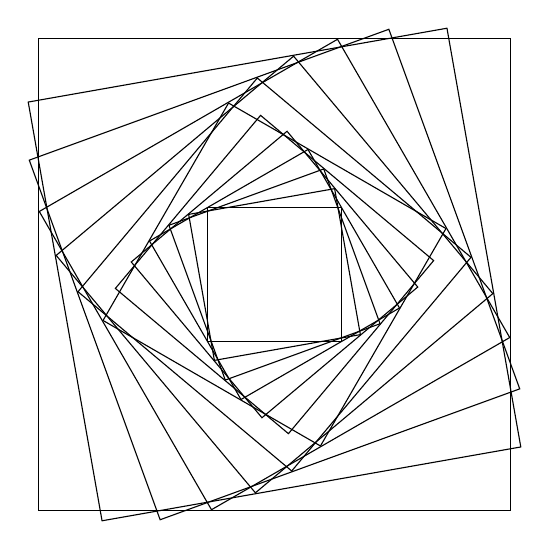
\begin{tikzpicture}
		\draw (-3, -3) rectangle (3, 3);
		\draw [scale = 0.9, rotate = 10] (-3, -3) rectangle (3, 3);
		\draw [scale = 0.9^2, rotate = 20] (-3, -3) rectangle (3, 3);
		\draw [scale = 0.9^3, rotate = 30] (-3, -3) rectangle (3, 3);
		\draw [scale = 0.9^4, rotate = 40] (-3, -3) rectangle (3, 3);
		\draw [scale = 0.9^5, rotate = 50] (-3, -3) rectangle (3, 3);
		\draw [scale = 0.9^6, rotate = 60] (-3, -3) rectangle (3, 3);
		\draw [scale = 0.9^7, rotate = 50] (-3, -3) rectangle (3, 3);
		\draw [scale = 0.9^8, rotate = 40] (-3, -3) rectangle (3, 3);
		\draw [scale = 0.9^9, rotate = 30] (-3, -3) rectangle (3, 3);
		\draw [scale = 0.9^10, rotate = 20] (-3, -3) rectangle (3, 3);
		\draw [scale = 0.9^11, rotate = 10] (-3, -3) rectangle (3, 3);
		\draw [scale = 0.9^12] (-3, -3) rectangle (3, 3);
	\end{tikzpicture}



\fontspec{SourceCodePro-Regular}
\lstset{
	language=[latex]tex,tabsize=4,
	moredelim=*[s][\itshape]{$}{$},
	moredelim=*[s][\color{red!40!.}]{(}{)},
	moredelim=*[s][\color{green!30!.}]{[}{]},
	backgroundcolor=\color{blue!5},
	commentstyle=\color{.!80}\itshape,
	texcsstyle=*\color{blue!40!.},
	moretexcs={
		draw,
	},
	deletetexcs={},
}
\lstinputlisting{transform2.tex}

\end{document}